\documentclass[12pt]{article}
\usepackage[utf8]{inputenc}
\usepackage[cyr]{aeguill}
\usepackage[french]{babel}
\usepackage{xspace}
\usepackage[T1]{fontenc}
\usepackage[dvipsnames]{xcolor}
\usepackage{url}
\usepackage{graphicx}
\usepackage{hyphenat}
\usepackage[left=15mm, right=15mm]{geometry}
\geometry{
    a4paper,
    total={170mm,257mm},
    top=30mm,
 }
\usepackage{csquotes}
\usepackage{bookmark}
\usepackage{biblatex}
\usepackage{listings}
\usepackage{hyperref}
\usepackage{subcaption}
\usepackage{fancyhdr}
\hypersetup{
    hidelinks,
}
\usepackage{eurosym}

\addbibresource{rapport.bib}

\lstset{
  aboveskip=3mm,
  belowskip=-2mm,
  backgroundcolor=\color{lightgray},
  basicstyle=\footnotesize,
  breakatwhitespace=false,
  breaklines=true,
  captionpos=b,
  commentstyle=\color{ForestGreen},
  deletekeywords={\ldots},
  escapeinside={\%*}{*)},
  extendedchars=true,
  framexleftmargin=16pt,
  framextopmargin=3pt,
  framexbottommargin=6pt,
  frame=tb,
  keepspaces=true,
  keywordstyle=\color{blue},
  language=Python,
  literate=
  {²}{{\textsuperscript{2}}}1
  {⁴}{{\textsuperscript{4}}}1
  {⁶}{{\textsuperscript{6}}}1
  {⁸}{{\textsuperscript{8}}}1
  {€}{{\euro{}}}1
  {é}{{\'{e}}}1
  {è}{{\`{e}}}1
  {ê}{{\^{e}}}1
  {ë}{{\¨{e}}}1
  {É}{{\'{E}}}1
  {Ê}{{\^{E}}}1
  {û}{{\^{u}}}1
  {ù}{{\`{u}}}1
  {â}{{\^{a}}}1
  {à}{{\`{a}}}1
  {á}{{\'{a}}}1
  {ã}{{\~{a}}}1
  {Á}{{\'{A}}}1
  {Â}{{\^{A}}}1
  {Ã}{{\~{A}}}1
  {ç}{{\c{c}}}1
  {Ç}{{\c{C}}}1
  {õ}{{\~{o}}}1
  {ó}{{\'{o}}}1
  {ô}{{\^{o}}}1
  {Õ}{{\~{O}}}1
  {Ó}{{\'{O}}}1
  {Ô}{{\^{O}}}1
  {î}{{\^{i}}}1
  {Î}{{\^{I}}}1
  {í}{{\'{i}}}1
  {Í}{{\~{Í}}}1,
  morekeywords={*,self, \_\_init\_\_, \_\_eq\_\_, \_\_str\_\_},
  numbers=left,
  numbersep=10pt,
  numberstyle=\tiny\color{black},
  rulecolor=\color{black},
  showspaces=false,
  showstringspaces=false,
  showtabs=false,
  stepnumber=1,
  stringstyle=\color{ForestGreen},
  tabsize=4,
  title=\lstname,
}

\title{
	\Huge
	\textbf{Développement d'une méthode de recherche arborescence pour un jeu à deux joueurs:
		application au jeu 7 Wonder-Duel}
	\vspace{0.4cm}

	\LARGE
	TER
}

\author{
	Cambresy Florian \\
	Chalaud Jean-Christophe \\
	Le Denmat Mickael
}

\begin{document}
	\newpage
	\begin{titlepage}
    \begin{center}
        \vspace*{1cm}

        \Huge
        \textbf{Développement d'une méthode de recherche arborescence pour un jeu à deux joueurs:
            application au jeu 7 Wonder-Duel}

        \vspace{0.4cm}
        \LARGE
        TER

        \vspace{1.6cm}

        \large
        CAMBRESY Florian \\
        CHALAUD Jean-Christophe \\
        LE DENMAT Mickaël \\

        \vfill
        
        \vspace{0.8cm}
        
\includegraphics[width=0.32\textwidth]{images/USVQ-logo.png}

        \vspace{0.4cm}

        \Large
        Université de Versailles Saint-Quentin-en-Yvelines \\
        \vspace{0.4cm}
        24 Mai 2020
    \end{center}
\end{titlepage}
    \pagestyle{fancy} 
    \fancyhead[L]{TER - 7 Wonder-Duel}
    \fancyhead[R]{\thepage}
    \fancyhead[C]{}
    \fancyfoot[C]{}
	\newpage
	\renewcommand{\contentsname}{Table des matières}
	\tableofcontents

	\newpage
	\section{Développement d'une méthode de recherche arborescence pour un jeu à deux joueurs:
	application au jeu 7 Wonder-Duel}
	\subsection{Sujet}
    	Il s’agira tout d’abord pour les étudiants de se familiariser avec les méthodes de recherche arborescente appliquées aux jeux, en particulier la méthode alpha-bêta. \\
    	Dans un second temps, il conviendra d'implémenter une telle méthode pour le jeu intitulé 7wonders - Duel.Ce jeu est décrit sur de nombreux sites, certains proposent même une petite vidéo tutorielle expliquant les règles de ce jeu. Il est à noter que l’encadrant offrira ce jeu aux étudiants qui
    	choisiront ce sujet. \\
    	Pour que le programme “joue bien”, il conviendra en particulier de réfléchir à des fonctions d'évaluation pertinentes des positions de jeu.

	\subsection{Description du travail attendu}
    	L'objectif du projet est d'implémenter une fonction d'évaluation ainsi que la méthode alpha-bêta pour faire en sorte qu'un algorithme puisse jouer. Ce dernier va prendre en entrée une situation de départ, c'est-à-dire les cartes de chaque joueur, leurs monnaies, et en sortie renvoie le coup à jouer. De plus ce coup doit être pertinent et digne d'intérêt. Nous discuterons de cette définition par la suite. Afin d'apporter une solution à ce sujet, nous découperons le projet en trois parties.
    	La première sera une partie descriptive concernant les notions contenues dans la méthode alpha-bêta pour que le programme joue correctement en insistant sur les points qui devront être étudiés afin d'appliquer la méthode à notre exemple précis. Ensuite, nous expliquerons les règles du jeu et évoquerons le déroulement d'une partie. Nous développerons le système de victoire et, afin de faire une transition sur la partie qui suivra, nous débattrons concernant la force des "positions" au cours d'une partie. La deuxième partie montrera le chemin de pensée que nous avons eu afin d'arriver à une ou des solutions pour appliquer la méthode alpha-beta sur notre jeu. Plus particulièrement nous décrirons la fonction d'évaluation que nous avons trouvé afin que l'algorithme suggère des coups pertinents. Enfin la dernière sera une présentation des solutions techniques que nous avons mise en place.

	\subsection{Description du jeu : 7 wonders-Duel}
    	7 Wonder est un jeu de plateau sorti dans les années 2010, créé par Antoine Bauza et publié par Repos Production en Belgique. Le nombre de joueurs est entre 3 et 7. On y joue une ancienne
    	civilisation avec ses conflits militaires mais aussi ses activites commerciales. Il est connu et très apprécié par la communauté ayant remporté plus de 30 prix et souvent cité comme l'un des jeux de société les plus influents de la dernière décennie\cite{wiki_7_wonder}. Le jeu choisi afin d'appliquer l'algorithme min-max est une variante de celui-ci, le 7 wonders - Duel.

	\subsubsection{7 wonders - Duel}
    	Le jeu 7 wonders - Duel est comme son nom l'indique un 7 wonders mais à deux joueurs. Un jeu sorti en 2015 par la même société.
    
    	\subsubsection{Règles du jeu}
    	Le jeu se présente comme suit dans le livret des règles\cite{regle_7_wonder_duel}.
    
        \begin{figure}[htbp]
            \centering
            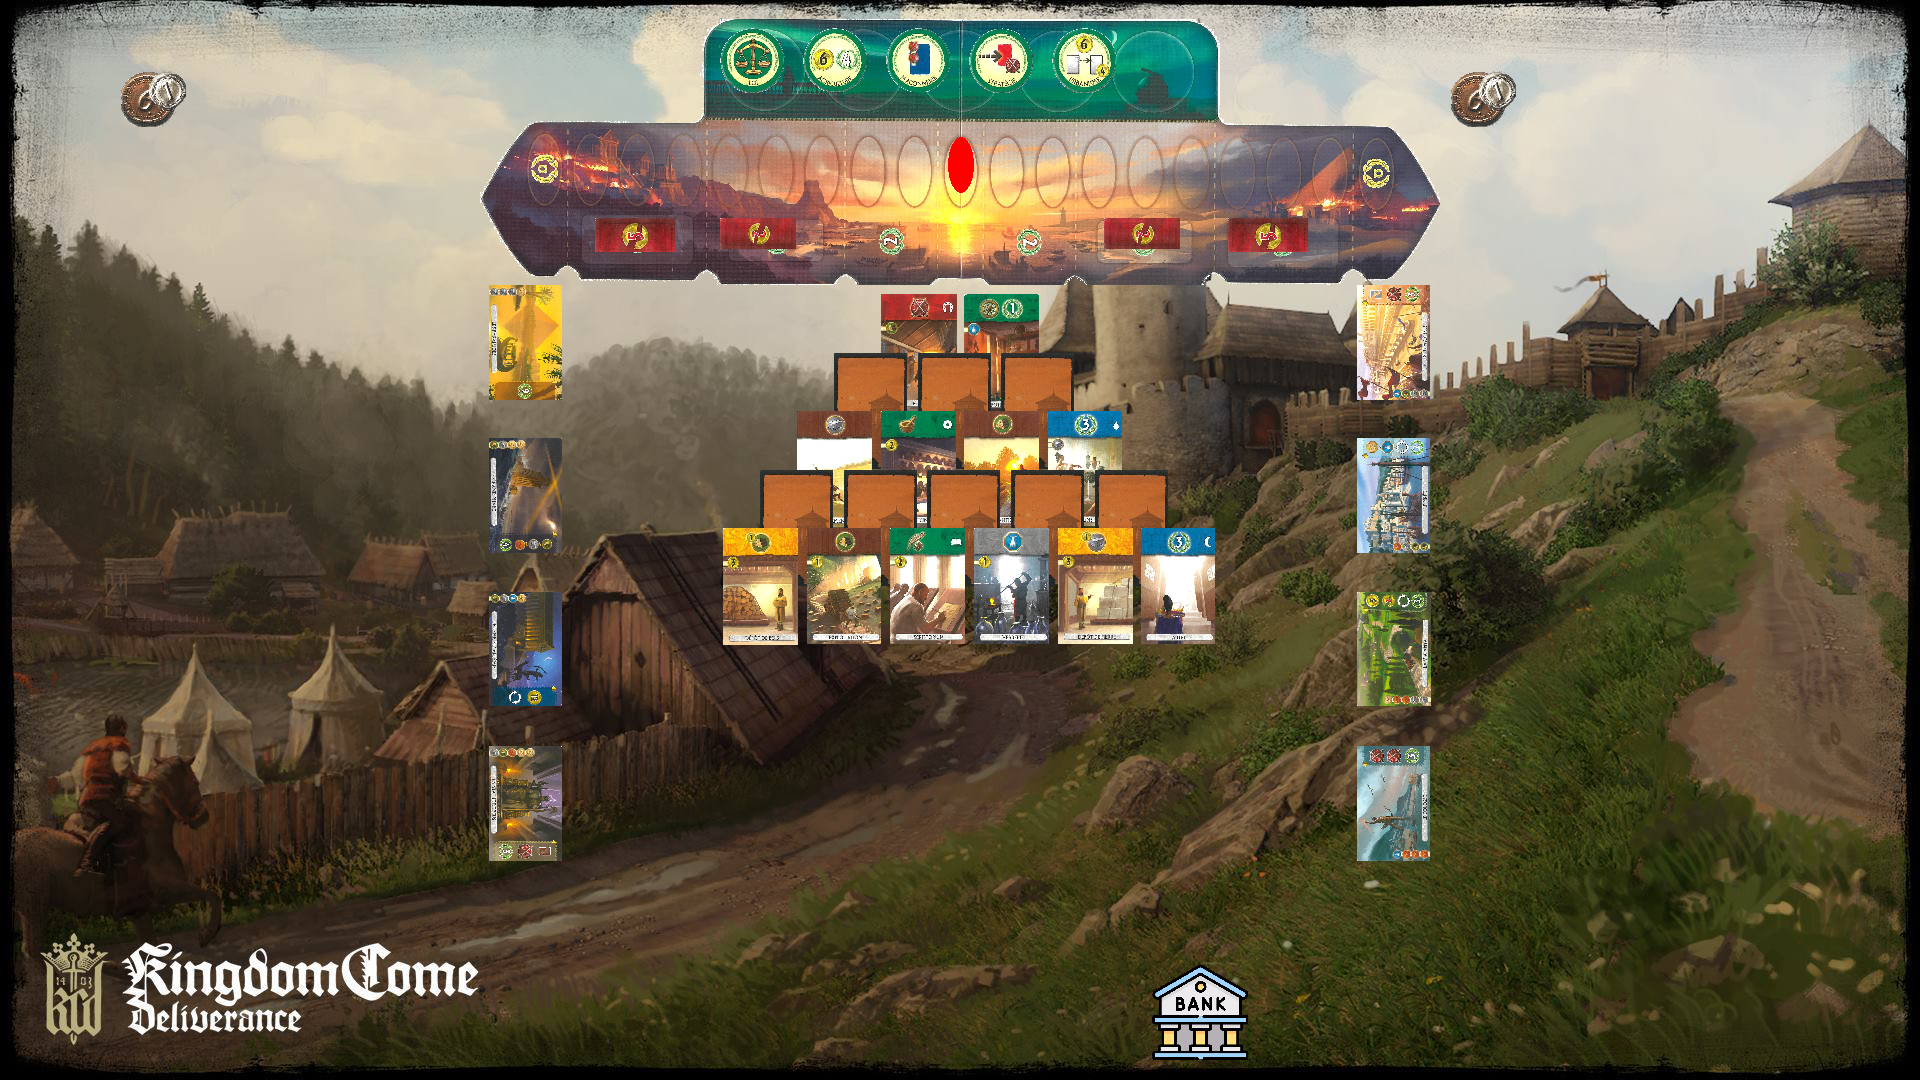
\includegraphics[width=.9\linewidth]{images/plateau_debut.png}
            \caption{Interface graphique}
            \label{fig:interface_graphique}
        \end{figure}
    
    	Il est constitué de:
    	\begin{itemize}
    		\item[-] 1 plateau de jeu.
    		\item[-] 66 cartes Âge.
    		\begin{itemize}
    			\item[+] 23 cartes pour l'Âge I.
    			\item[+] 23 cartes pour l'Âge II.
    			\item[+] 20 cartes pour l'Âge III.
    		\end{itemize}
    		\item[-] 7 cartes Guilde.
    		\item[-] 12 cartes Merveille, avec un nom, un coût en ressource et un effet (un bonus).
    		\item[-] 4 jetons Militaire, donnant une certaine somme de monnaie.
    		\item[-] 10 jetons Progrès.
    		\item[-] 1 Pion Conflit, indiquant quel joueur a l'avantage militaire.
    		\item[-] 31 pièces de monnaie
    		\begin{itemize}
    			\item[+] 14 de valeur 1.
    			\item[+] 10 de valeur 3.
    			\item[+] 7 de valeur 6.
    		\end{itemize}
    		\item[-] 1 carnet de scores.
    	\end{itemize}
    
    	Les cartes Âge et Guilde sont des bâtiments. Elles peuvent avoir un coût (monetaire) afin d'être
    	utilisées, qui est placé en haut à gauche. Elles peuvent donner des effets, placé en haut au centre.
    	Les effets sont multiples comme par exemple une production de matière, une réduction de coût de construction d'un bâtiment ou d'une merveille, ainsi que d'autres. Enfin elles ont aussi un nom, placé en bas. Les cartes ont des couleurs différentes indiquant à quel type de bâtiment elles appartiennent.
    	\begin{itemize}
    		\item[•] Les Cartes marrons sont des bâtiments de matière première.
    		\item[•] Les Cartes grises sont des bâtiments de produit manufacturé.
    		\item[•] Les cartes bleues sont des bâtiments civils, elles donnent des points de victoire.
    		\item[•] Les cartes vertes sont des bâtiments scientifiques, elles donnent aussi des points de victoire et
    		\item[•] Un symbole scientifique. Lorsqu'un joueur a deux symboles scientifique identique
    		il peut prendre un jeton Progres.
    		\item[•] Les cartes oranges sont des bâtiments commerciaux, elles ont des objectifs multiples comme donner
    		des pièces au joueur, produire des ressources, modifier les règles de commerce.
    		\item[•] Les cartes rouges sont des bâtiments militaires, elles augmentent la puissance.
    		\item[•] Les cartes violettes sont des bâtiment de Guilde, elles donnent des points de victoire en fonction
    		de certains critères.
    	\end{itemize}
    
    	De plus le joueur peut acheter des ressources à la "banque" via le commerce comme par exemple si le joueur souhaite construire un bâtiment mais ne dispose pas de toutes les ressouces. Pour acheter cette ressource il faut prendre en compte les ressources produites par le joueur adverse (carte marron et grise) y ajouter 2 et remettre la somme dans la banque puis construire le bâtiment. Concernant les bâtiments, certains octroient un symbole de chaînage (en blanc en haut de la carte). Si le joueur souhaite construire un bâtiment et si il possède une carte donnant le symbole de chaînage il peut alors le construire gratuitement, dans le cas contraire il doit payer son coût en ressources et/ou monetaire.
    
    	Une fois la présentation faite, nous allons pouvoir parler de la préparation du jeu avant de débuter une partie.
    	La préparation du plateau se fait ainsi:
    	\begin{enumerate}
    		\item Placez le plateau entre les deux joueurs.
    		\item Placez le pion Conflit sur la case neutre au milieu du plateau.
    		\item Placez les quatres jetons Militaire sur leurs emplacements.
    		\item Mélangez les jetons Progrès et placez-en cinqs au hasard sur la plateau.
    		\item Chaque joueur prend 7 pièces à la banque.
    	\end{enumerate}
    
    	Puis vient la selection des Merveilles, pour cela il faut désigner le premier joueur et mélanger les Merveilles,
    	ensuite:
    	\begin{itemize}
    		\item Disposez 4 Merveilles aléatoires entre les joueurs.
    		\item Le premier joueur choisit une Merveille.
    		\item Le deuxième joueur en choisit deux.
    		\item Le premier joueur prend la dernière.
    		\item Disposez les quatres autres Merveilles.
    		\item Le deuxième joueur choisit une Merveille.
    		\item Le premier joueur en choisit deux.
    		\item Le deuxième joueur prend la dernière.
    	\end{itemize}
    	Pour construire une Merveille, le joueur doit mettre une carte face cachée sous la Merveille (peu importe la carte, elle sert juste a indiquer que la Merveille est construite) et doit payer le coût de la construction. Il y a un maximum de sept Merveilles construit par partie, le joueur dont la dernière Merveille n'est pas construite doit la remettre dans la boite.\\
    	Enfin il faut placer les cartes d'Âge dans une structure particulière en fonction de l'âge. Les cartes face cachées sont retournées lorsque les cartes visibles posées dessus sont enlevées par les joueurs. Les joueurs peuvent choisir aussi de défausser une carte en échange de 2 pièces et d'un bonus d'une pièce pour chaque carte jaune qu'il possède.
    
    	Il y a trois manières de gagner, la première est la victoire militaire, l'un des joueur aura avancé le pion Conflit dans la case capitale de son adversaire. La deuxième étant la victoire par suprémactie scientifique, l'un des joueurs réunit 6 symboles scientifiques différents. Enfin, si aucun des joueurs n'a gagné à la fin de l'Âge III, il faut alors faire la sommes des points de victoire acquis durant la partie, celui qui en possde le plus l'emporte.

	\section{Rappels généraux}
	\subsection{Théorie des jeux}
    	Dans le monde des mathématiques il y a un domaine qui s'intéresse aux interactions stratégiques qui existent entre plusieurs agents. Ces interactions peuvent se faire dans un jeu, dans les sciences sociales, politiques ainsi que dans d'autres exemples. Ce domaine est la théorie des jeux\cite{wiki_theorie_jeux}. Il faut noter que ici le mot "jeu" a un sens plus large qu'un jeu de société ou autre. Dans ce projet nous porterons attention uniquement aux interactions entre deux joueurs dans un jeu de société à travers un exemple que nous développerons par la suite.

	\subsection{Catégories de jeux}
    	Afin de connaître quelle approche doit être utilisée pour étudier les stratégies qui existent au sein d'un jeu, la théorie repartie les jeux en différentes catégories\cite{wiki_typo_theorie_jeux}.
    	\begin{enumerate}
    		\item Coopératifs ou non.
    		\item Somme nulle ou non.
    		\item Simultanés ou séquentiels.
    		\item Information complète ou non.
    		\item Mémoire parfaite ou non.
    		\item Determiné.
    		\item Finis.
    		\item Répétés.
    	\end{enumerate}
    	(1) Un jeu coopératif permet d'analyser la formation de coalitions afin d'améliorer le gain potentiel. \\
    	(2) Un jeu à somme nulle (ou jeu strictement compétitif) est un jeu dont les gains de certains joueurs sont les pertes des autres afin d'avoir la somme des gains et des pertes nulle, comme dans les échecs, dans le poker ou dans d'autres. A l'inverse dans un jeu à somme non nulle, tous les joueurs peuvent perdre, ou gagner, voir même certains peuvent gagner un gain moins (réciproquement plus) important que la perte totale d'autres joueurs.\\
    	(3) Un jeu est dit "simultané" si les joueurs jouent en même temps, dans le cas contraire c'est un jeu séquentiel.\\
    	(4) Un jeu peut être à "information complète", c'est-à-dire que chaque joueur connait l'ensemble des informations qui influent leur prise de décision.\\
    	(5) Un jeu peut être aussi à "mémoire parfaite", dans ce cas chaque joueur peut se rappeler des coups qui ont été joués soit en les notant a part, soit ils sont visibles au cours de la partie (par exemple les cartes qu'a choisie le joueur sont à coté de ce dernier, face visible).\\
    	(6) Un jeu "déterminé" est un jeu particulier à somme nulle sans intervention du hasard.

	\subsection{Représentation d'un jeu}
    	Maintenant que nous savons comment définir un jeu, nous allons étudier comment représenter ce dernier et les interactions entre les joueurs. Il existe globalement trois représentations\cite{wiki_representation_theorie_jeux}, la forme extensive et la forme normale, qui sont utilisées pour les jeux non coopératifs et la forme caractéristique pour les jeux coopératifs.

	\subsubsection{forme extensive}
    	La forme extensive est la représentation sous forme d'arbre de décision où les noeuds d'une même hauteur sont les choix possibles (qui ne sont pas en dehors des règles prévues par le jeu) d'un joueur. Plus précisément chaque noeud est une situation produite au cours d'une partie (pas nécessairement le début de la partie) et les fils de ce noeud sont les coups que peut faire le joueur suivant. Par exemple dans les échecs, la racine sera l'état du plateau de jeu à la fin du tour d'un joueur (la position des pions de chaque joueur) et les fils de cette racine seront les déplacements des pions de l'adversaire. Dans cet exemple, ainsi que dans tous les jeux à deux joueurs, les hauteurs paires sont les coups du joueur A tandis que les hauteurs impaires sont les coups du joueur B. De plus, les feuilles de cet arbre sont des noeuds indiquant la fin de la partie, soit il y a victoire d'un des deux joueurs, soit plus aucun coup n'est possible.
    	C'est la forme que nous allons utiliser durant tout ce projet, c'est pour cela que nous passerons rapidement sur les autres formes.

	\subsubsection{forme normale}
    	La forme normale (ou stratégique) est définie par:
    	\begin{itemize}
    		\item[°] L'ensemble des joueurs (de taille finie).
    		\item[°] L'ensemble des stratégies possibles pour chacun des joueurs (fini ou infini).
    		\item[°] Les préférences de chacun des joueurs, soit un sous-ensemble de stratégies parmi l'ensemble des
    		\item[°] combinaisons stratégiques possibles soit via une fonction d'utilité ou un fonction de gain.
    	\end{itemize}

	\subsubsection{forme caractéristique}
    	La forme caractéristique est utilisée, comme dit précédememnt, pour les jeux coopératifs. Elle est représentée sous forme d'un graphe G=(N,v) avec N l'ensemble des joueurs et v la fonction caractéristique. Cette dernière associe à chaque sous-ensemble de joueurs (noté S) qui forme une coalition, la valeur v(S), la gain obtenu par la coalition.

	\subsection{Recherche arborescente et intelligence artificielle}
    	La recherche arborescente est une recherche qui se base sur la forme extensive afin d'utiliser l'arbre de décision\cite{cours_arbre_decision}. Cette recherche s'appuie aussi sur une fonction d'évaluation, qui associe à toutes situations du jeu une valeur indiquant si elle est favorable à une victoire. Bien évidemment plus cette valeur est grande plus la probabilité de victoire est grande. Cette fonction ne s'applique qu'aux feuilles de l'arbre de décision, ces feuille peuvent être la fin de la partie ou un état de la partie dans lequel nous évaluons le rapport de force
    	entre les deux joueurs afin de déterminer qui est en meilleur posture pour gagner. Ainsi l'objectif de cette recherche est de choisir la suite de noeud à prendre (donc de coups à faire) afin d'arriver à la valeur d'évaluation maximale.

	\subsection{Méthode alpha-bêta}
	\subsubsection{Méthode min-max}
    	Avant d'évoquer la méthode alpha-bêta, nous allons expliquer comment fonctionne la méthode min-max,
    	la méthode alpha-bêta en est une amélioration. La méthode min-max est un algorithme utilisé dans la théorie des jeux, plus précisément dans les jeux à deux joueurs, à somme nulle et à information complète\cite{min_max}. L'objectif de cette dernière est de minimiser la perte dans le pire cas pour un joueur est de maximiser la perte pour l'adversaire, d'où son nom "min-max". Pour cela l'algorithme va simuler tous les coups possibles et leur donner une valeur, représentant combien ce coup est intéressant ou non. La simulation de tous les coups possibles passe par la construction de l'arbre de décision et le calcul de la valeur des feuilles est l'application d'une fonction d'évaluation. Nous obtenons donc un arbre avec des valeurs aux feuilles uniquement. Ensuite, nous allons devoir faire "remonter" la valeur du jeu des feuilles jusqu'à la racine et choisir parmi tous les coups celle qui a la valeur la moins basse. Pour calculer cette valeur nous allons passer par une approche récursive comme suit\cite{minimax_alog}:
	
    	\begin{itemize}
    		\item minmax(p) = f(p) si p est un feuille de l'arbre où f est la fonction d'évaluation.
    		\item minmax(p) = max(minmax(O$_1$), \ldots, minmax(O$_n$)) si p est un noeud de l'ordinateur avec les
    			fils O$_1$, \ldots, O$_n$.
    		\item minmax(p) = min(minmax(O$_1$), \ldots, minmax(O$_n$)) si p est un noeud du joueur avec les fils
    			O$_1$, \ldots, O$_n$.
    	\end{itemize}
    
    	Le souci de cette méthode est le nombre de cas à étudier. En effet comme la simulation
    	produit un arbre que nous devons parcourir en entier afin de choisir le meilleur coup à jouer
    	nous devons faire un parcours de cet arbre. Cependant comme cela passe soit par un algorithme récursif,
    	qui doit simuler un nombre important de coups et de réponses ce qui fait augmenter la profondeur de l'arbre.
    	En plus de faire augementer le nombre d'appels récursifs cela surcharge le tas d'appel. Soit, dans l'autre cas,
    	nous pouvons passer par un algorithme itératif avec une file ou une pile. Or si le nombre de réponses possibles
    	à un coup du joueur devient trop important cela nous oblige à utiliser beaucoup de mémoire. Enfin, même si nous
    	prévoyons le fait que le programme utilise beaucoup de mémoire, nous ne voulons pas que le programme continue de
    	calculer une suite de coups qui est moins avantageuse une suite qu'il à déjà calculé. Cela serai contre-productif.
    	Ainsi c'est pour répondre à toutes ces problématiques que l'élagage alpha-bêta a été conçu.

	\subsubsection{Amélioration alpha-bêta}
    	L'élagage alpha-bêta est comme son nom l'indique une méthode qui vise à "supprimer" les branches de l'arbre qui
    	ne sont pas utiles, qui ne change rien au résultat final. Pour élager les branches, nous disposons de deux types de
    	coupures, la coupure alpha et la coupure bêta, d'où le nom de la méthode\cite{elagage_alpha_beta}
    	Cette méthode s'applique uniquement sur des arbres au moins de profondeur trois
    	(la racine ayant un profondeur de un). Une fois que la méthode min-max à construit l'arbre
    	et appliqué la fonction d'évaluation aux feuilles, nous allons ajouter les coupures lors de la
    	"remonter" des valeurs à la racine.

	\subsubsection{Coupure Alpha}
	    \label{coupure_alpha}
	    \begin{figure}[htbp]
            \centering
            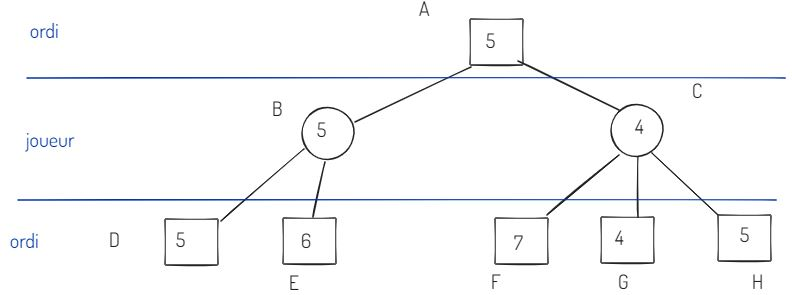
\includegraphics[width=.8\linewidth]{images/elagage_alpha.JPG}
            \caption{Elagage alpha (1) (exemple ici de : \cite{elagage_alpha_beta})}
            \label{fig:elagage_alpha}
        \end{figure}
    
    	Prenons l'exemple ci-dessus pour expliquer la coupure alpha, elle se place du point de vue du joueur. Une fois que la valeur du noeud B à été initialisé avec le minimum de ces fils (D, F) cette valeur va nous servir de borne pour faire nos coupures. Regardons les fils du frère de B, c'est à dire F, G (supposons que la valeur de H ne soit encore connue) afin d'initialiser la valeur de C. Nous devons prendre la valeur minimale entre F et G (ici F=4) mais nous constatons que cette valeur est plus petite que notre borne (B=5), ainsi explorer le noeud H ne sert a rien car peut importe la valeur qu'il aura (plus petite ou plus grande que F) il ne sera pas
    	utiliser pour initialiser la valeur de A pusique A=max(B,C). Nous pouvons donc élaguer H (et tous les autres fils
    	de C s'ils existent) comme sur l'image ci-dessous.
    
    	\begin{figure}[htbp]
            \centering
            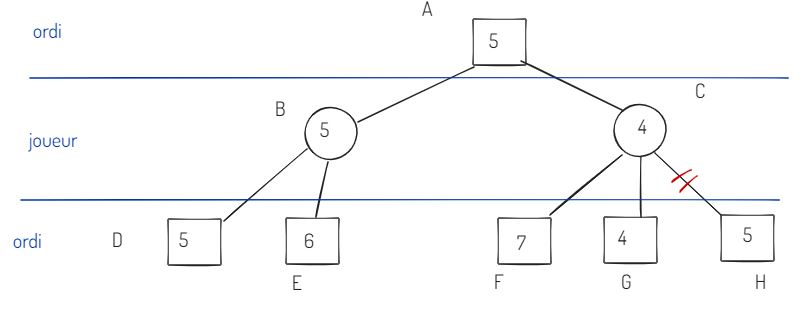
\includegraphics[width=.8\linewidth]{images/elagage_alpha_suite.JPG}
            \caption{Elagage alpha (2) (exemple ici de : \cite{elagage_alpha_beta})}
            \label{fig:elagage_alpha_suite}
        \end{figure}

	\subsubsection{Coupure Bêta}
	    \label{coupure_beta}
    	La coupure bêta est similaire mais se base du point de vue de l'ordinateur, on élague donc les
    	feuilles plus grande que la borne \cite{wiki_7_wonder}.

	\section{Travail effectué}
	\subsection{La fonction d'évaluation}
    	Comme expliqué précédememnt la fonction d'évaluation nous permet d'associer un nombre à une situation lors d'une partie. C'est-à-dire l'ensemble des éléments (cartes, merveilles, monnaies, position du jeton conflit, jetons militaires, jetons progrès) présents sur le plateau. Pour cela nous avons commencé par réduire le nombre d'éléments que nous prenons en compte lors d'une partie et nous avons travaillé uniquement avec les cartes. De plus nous avons considéré uniquement les cartes de l'age I. Après quelques brain storming nous avons conclu que la solution la plus simple était de donner un "poids" aux cartes en fonction de notre manière de jouer, puis de modifier ce poids en fonction de la situation. \\
    
    	Pour définir ce poids, nous nous sommes tous reunis afin de nous concerter pour trouver la note la plus adequate pour chacune des cartes. Premièrement nous avons défini un intervalle de valeur arbitraire (entre 0 et 20) et nous avons aussi attribué un poids à une carte face cachée (la moyenne de l'intervalle donc 10). Pour les cartes avec une valeur	inférieure à 10, il est préférable de tenter de prendre la carte face cachée, avec une chance de 50 \% d'avoir une meilleure carte. De cette manière nous avons pu prendre en compte l'évolution des âges au cours d'une partie. Nous avons défini un objectif par âge, le premier doit permettre au joueur de collecter des ressources simples donc du bois, de la pierre et de l'argile. L'âge II doit permettre au joueur de collecter des ressources rares, donc verre et papyrus mais aussi attaquer et obtenir des symboles scientifiques et construire des merveilles. Durant le dernier âge le joueur doit viser les cartes donnant des points militaires. Cette solution nous permet aussi de prendre en compte le coût des cartes, par exemple les cartes "Chantier" et "Exploitation" donnent toutes les deux du bois mais "Exploitation" coûte une pièce, si nous avons le choix entre les deux il est préférable de prendre "Chantier" et d'utiliser la monnaie pour acheter des ressources que nous ne possédons pas. \\
    	
    	\begin{figure}[htbp]
    	    \centering
    	    \begin{subfigure}{.3\textwidth}
                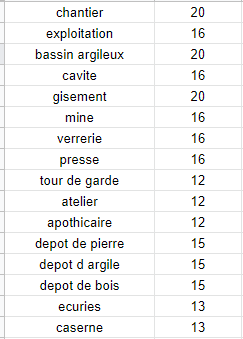
\includegraphics[width=.9\linewidth]{images/notation_cartes.PNG}
    	    \end{subfigure}
    	    \begin{subfigure}{.3\textwidth}
                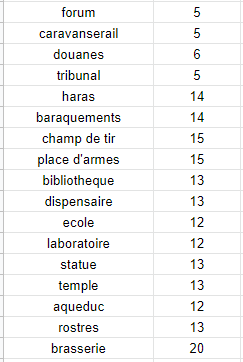
\includegraphics[width=.9\linewidth]{images/notation_cartes2.PNG}
    	    \end{subfigure}
    	    \begin{subfigure}{.3\textwidth}
                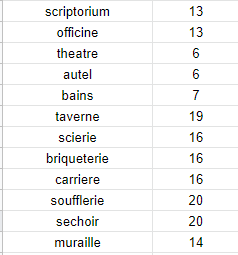
\includegraphics[width=1.1\linewidth]{images/notation_cartes3.PNG}
    	    \end{subfigure}
    	    \caption{Exemple de notation de carte}
        \end{figure}
    
    	Après plusieurs parties contre l'ordinateur, nous avons ajouté la possibilité de construire des merveilles. Nous avons utilisé la même méthode évoquée précédemment.
    
    	% TODO : à finir

    \newpage
	\subsection{Implémentation}
	Pour l'implémentation nous avons décidé de commencer par réfléchir au découpage du jeu
	en différent modules ainsi que du design de l'interface.

	Nous avons conclus que l'arborescence des fichiers serait:
	\begin{itemize}
		\item[-] Un dossier "interface\_graphique" contenant tous les fichiers utiles pour l'interface graphique, c'est-à
		-dire :
		\begin{itemize}
			\item[+] Un dossier "ressources" avec toutes les images (cartes, merveilles, jetons, plateau, \ldots). Mais
			aussi les musiques.
			\item[+] Un dossier "src" contenant les fichiers sources de l'interface, c'est-à-dire :
			\begin{itemize}
				\item[.] Boutons.py
				\item[.] Constantes.py
				\item[.] Fenetre.py
				\item[.] MonSprite.py
				\item[.] SpriteCarte.py
				\item[.] SpriteJetonMilitaire.py
				\item[.] SpriteJetonProgre.py
				\item[.] SpriteMerveille.py
			\end{itemize}
		\end{itemize}
		\item[-] Un dossier "utils" contenant tous les fichiers utiles au jeu, c'est-à-dire :
		\begin{itemize}
			\item[°] Carte.py
			\item[°] CarteGuilde.py
			\item[°] Merveille.py
			\item[°] JetonMilitaire.py
			\item[°] JetonProgres.py
			\item[°] Joueur.py
			\item[°] notation\_carte.cvs (un fichier stockant les "poids" des cartes)
			\item[°] Outils.py
			\item[°] Plateau.py
			\item[°] Stratégie.py
		\end{itemize}
		\item[-] Un dossier "test" contenant tous les fichiers tests, c'est-à-dire :
		\begin{itemize}
			\item[*] TestCarteJeton.py
			\item[*] TestJoueur.py
			\item[*] TestMerveille.py
			\item[*] TestPlateau.py
			\item[*] TestStratégie.py
		\end{itemize}
	\end{itemize}

	Comme vous pouvez le constater les extensions de fichiers sont en ".py" cela signifie que se sont des fichiers Python. En effet lorsque nous avons discuté au sujet du langage à utiliser nous avions remarqué qu'ils nous fallait un langage orienté objet et que nous maîtrisons. Nous avions donc le choix entre le Java et le Python. Pour des raisons de simplicité nous avons choisi le Python. Une fois tous les préparatifs terminés nous avons commencé l'implémentation à proprement parlé. Nous avons suivi plusieurs phases, nous travaillons sur un module, une fois fini nous le testons à travers différentes batteries de tests, puis nous passons au module suivant. Une fois le jeu fini nous avons testé le jeu en 1vs1 via le terminal. Nous allons maintenant expliquer brièvement le contenue des différentes classes constituant le projet et nous detaillerons le contenue de la classe "Stratégie" qui est le coeur du projet.

	\subsubsection{Carte}
		Commençons par la classe carte.
		Une carte est composé d'un nom, d'un effet, d'un cout, d'un nom de carte de chainage (none si la carte n'en possède pas), une couleur, et elle appartient à un age.
		Concernant les effets et les couts, nous avons utilisé les propriétés du Python en définissant les effets comme des chaînes de caractère respectant un pattern précis. Elle commencent par le type d'effet comme "ressource", "monnaie", "attaquer", "symbole\_scientifique" puis les paramètres comme "ressource bois 1", "attaquer 3". Les classe "CarteGuilde" et "Merveille" sont des classes filles de la classe "Cartes". Les cartes guildes et les merveilles sont des cartes mais sans carte de chaînage sans couleur et sans âge (elles appatiennent toutes à l'âge III). Les merveilles possèdent un attribut pour savoir si elles sont construit ou non.

	\subsubsection{Jetons}
		Passons maintenant aux jetons. Il en existe deux types, le jeton militaire qui possède un nom, un nombre de pièces que perd l'adversaire lorsque le jeton est pris et un nombre de points de victoire que gagne le joueur. Le deuxième type est le jeton progrès qui possède un nom et des effets.

	\subsubsection{Joueur}
		Nous avons aussi une classe joueur. Le joueur est définit par un nom, et possède plusieurs listes d'objets visible sur le plateau, c'est-à-dire ces cartes, ces meveilles, et ces jetons progrès, ainsi  que de la monnaie. Mais aussi d'autre informations comme un dicionnaire de ressource, des points de victoires un dicionnaire de symbole scientifiques et le nombre de symbole scientifiques différent. Cette classe implémente certaines méthodes qui le jeu utilise pour avoir des informations comme par exemple les coûts manquants pour construire une carte, dans ce cas il faut regarder dans le dicionnaire de ressource du joueur, mais aussi ces monnaies ainsi que dans ces merveilles ou cartes la présence de carte donnant des ressources au choix ou d'autre effet impliquant la construction de carte ou de merveille. Il existe aussi d'autres méthodes comme savoir si le joueur possède une carte pour faire du chaînage , s'il produit un type de ressources en particulier, ect\ldots.

	\subsubsection{Plateau}
		Toutes les différentes fonctionnalitées du jeu sont dans le fichier Plateau.py. Cette classe
		représente le jeu dans sa globalité c'est-à-dire le plateau avec les jetons progrès choisit,
		les cartes présentent en dessous du plateau, les deux joueurs, la fausse et la banque.
		Elle s'occupe aussi des effets des cartes ainsi que des effets des merveilles.
		C'est aussi la première classe que nous avons developpé durant le projet, elle a donc connue
		plusieurs évolutions.\\
		La classe Plateau contient toutes les méthodes faisant fonctionner le jeu. Elle 
		implémente une méthode pour préparer le plateau, c'est-à-dire
		tirer aléatoirement les jetons, les cartes, ainsi que les merveilles (si le jeu
		est en mode choix automatique). Elle contient aussi des méthodes pour piocher, 
		pour enlever une carte, pour obtenir la liste des cartes prenables, pour intéragir
		avec la banque, ect \ldots.\\
		Après tout cela, l'équipe se sépare en deux groupes, l'un crée l'interface pendant que l'autre fait l'algorithme minimax, d'alpha beta ainsi que la fonction d'évaluation.

	\subsubsection{Stratégie}
		Concernant la classe "Stratégie", elle contient la fonction d'évaluation, la fonction
		minimax ainsi que son amélioration la fonction alpha-beta.
		Elle commence d'abord par lire le fichier contenant le poids des cartes, des merveilles, et des jetons progrès.
		
		\begin{lstlisting}
			notation_carte = {}
			with open("src/utils/notation_cartes.csv", mode='r') as file:
				fichier_cvs = csv.reader(file)
				for lignes in fichier_cvs:
					notation_carte[lignes[0]] = int(lignes[1])
		\end{lstlisting}
		
		Nous avons rempli un fichier Google Sheet avec le nom de la carte puis son poids. Puis nous l'avons importé sous un format rapide et simple à lire, le format csv. Le Python nous a permit d'éxecuter ceci en seulement quelques lignes de code. \\
		Nous avons ensuite la fonction d'évaluation, elle prend en entrée
		la partie à un instant donné et va renvoyé une valeur, la différence
		entre l'évalution du joueur 2, donc de l'ordinateur, et du joueur 1.

		\begin{lstlisting}
def fonction_evaluation(partie):
	evaluation_j2 = 0
	for carte in partie.joueur2.cartes:
		if carte.est_face_cachee:
			evaluation_j2 += 10
		else:
			evaluation_j2 += notation_carte[carte.nom]
	
	for merveille in partie.joueur2.liste_merveilles_construite():
		evaluation_j2 += notation_carte[merveille.nom]
	
	if partie.joueur1.monnaie == 0:
		evaluation_j2 += 10
					
	if partie.position_jeton_conflit == 0:
		evaluation_j2 += 10
	
	evaluation_j1 = 0
	for carte in partie.joueur1.cartes:
		if carte.est_face_cachee:
			evaluation_j1 += 10
		else:
			evaluation_j1 += notation_carte[carte.nom]
	
	for merveille in partie.joueur1.liste_merveilles_construite():
		evaluation_j1 += notation_carte[merveille.nom]
	
	if partie.joueur2.monnaie == 0:
		evaluation_j1 += 10
	
	if partie.position_jeton_conflit == 18:
		evaluation_j1 += 10
	return evaluation_j2 - evaluation_j1
		\end{lstlisting}

		Comme nous l'avons expliqué plutôt la fonction va parcourir les cartes du deuxième joueur et va faire la somme de leur poids. Puis elle va faire la somme du poids des merveilles construites. La fonction va de même pour le joueur un. Nous avons ajouté deux trois modifications, notamment si la position du jeton militaire est à 0, donc dans la ville du joueur 1, la situation est très favorable pour l'ordinateur
		est inversement. Nous ajoutons un poids pour indiquer que la situation est favorable. \\
		Enfin nous avons la fonction minimax et alpha-beta, nous sommes parties d'un tutoriel sur Youtube \cite{implementation_minimax_alpha_beta} que nous avons adapté avec notre jeu. La fonction minimax est une fonction récursive qui prend en paramètre l'état de la partie, la profondeur a calculé, un booléen indiquant si c'est à l'ordinateur de jouer et le nombre de noeuds. Elle renvoie l'évaluation du meilleur coup, la carte à prendre, et le nombre de noeuds évalués. \\
		Nous allons commencer par expliquer l'implémentation avec la version qui ne prend pas en compte les merveilles et les jetons progrès.
		\begin{lstlisting}
def minimax(partie, profondeur, coup_bot, nbr_noeuds):
	if profondeur == 0 or partie_fini(partie):
		return fonction_evaluation(partie), None, nbr_noeuds+1
	
	carte_a_prendre = None
	
	if coup_bot:
		partie.joueur_qui_joue = partie.joueur2
		max_eval = -math.inf
		
		for carte in partie.liste_cartes_prenables() [1]:
			
			copie_partie: Plateau = partie.constructeur_par_copie() [2]
			ret = copie_partie.piocher(carte) [3]
			
			if ret == -1:
				copie_partie.defausser(carte) [4]
			else:
				copie_partie.joueur_qui_joue.cartes.append(carte) [5]
				copie_partie.enlever_carte(carte) [6]
			
			evaluation, _, nbr_noeuds = minimax(copie_partie, profondeur - 1, False, nbr_noeuds) [7]
			
			if evaluation > max_eval: [8]
				max_eval = evaluation
				carte_a_prendre = carte
				
		return max_eval, carte_a_prendre, nbr_noeuds+1
	
	else:
		partie.joueur_qui_joue = partie.joueur1
		min_eval = math.inf
		
		for carte in partie.liste_cartes_prenables():
			
			copie_partie: Plateau = partie.constructeur_par_copie()
			copie_partie.piocher(carte)
			copie_partie.joueur_qui_joue.cartes.append(carte)
			copie_partie.enlever_carte(carte)
		
			evaluation, _, nbr_noeuds = minimax(copie_partie, profondeur - 1, True, nbr_noeuds)
			
			if evaluation < min_eval:
				min_eval = evaluation
				carte_a_prendre = carte
		
		return min_eval, carte_a_prendre, nbr_noeuds+1
		\end{lstlisting}

		Cette fonction permet de simuler le coup de l'ordinateur et le coup du joueur. Pour cela elle parcourt toutes les cartes prenables de la partie passée en paramètre [1], pour chacune d'entre elles, la fonction créer une copie de la partie [2]. Comme nous simulons un coup, nous apportons des modifications au jeu mais nous ne voulons pas que ces modifications soient appliquées sur le jeu original, nous sommes obligés de faire des copies profondes des objets puis de modifier les copies. Dans cette copie, le joueur (ou l'ordinateur) pioche une carte [3] (la fonction "piocher" applique les effets de la carte). Si c'est à l'ordinateur de jouer et qu'il ne possède pas les ressources suffisantes pour piocher alors il la défausse [4]. Sinon nous ajoutons la carte dans la liste des cartes qu'il a en main [5] et nous supprimons cette carte du plateau [6]. Une fois toutes ces étapes terminé, nous avons simulé un coup dans la partie, nous allons a présent simuler les réponses à ce coup en appelant la fonction récursivement [7]. Enfin nous mettons à jour le merilleur coup a jouer [8], si l'evaluation, c'est à dire la différence la plus grande (réciproquement plus petite) entre le coup actuel et toutes les réponses de l'adversaire et supérieure (réciproquement inférieure) avec la meilleur évaluation alors nous changons l'évaluation et nous changons la carte à prendre (à jouer). C'est avec cette suite d'appels récursifs que nous créeons l'arbre de décision.\\

		Passons maintenant à la version alpha-beta de la fonction.
		\begin{lstlisting}
def alpha_beta(partie, profondeur, alpha, beta, coup_bot, nbr_noeuds):
	if profondeur == 0 or partie_fini(partie):
		return fonction_evaluation(partie), None, nbr_noeuds+1
	
	carte_a_prendre = None
	
	if coup_bot:
		partie.joueur_qui_joue = partie.joueur2
		max_eval = -math.inf
		
		for carte in partie.liste_cartes_prenables():
			
			copie_partie: Plateau = partie.constructeur_par_copie()
			ret = copie_partie.piocher(carte)
			if ret == -1:
				copie_partie.defausser(carte)
			else:
				copie_partie.joueur_qui_joue.cartes.append(carte)
				copie_partie.enlever_carte(carte)
			
			evaluation, _, nbr_noeuds = alpha_beta(copie_partie, profondeur - 1, alpha, beta, False, nbr_noeuds)
			
			if evaluation > max_eval:
				max_eval = evaluation
				carte_a_prendre = carte
				
				alpha = max(alpha, evaluation) [1]
				if beta <= alpha: [2]
					break [3]
				
		return max_eval, carte_a_prendre, nbr_noeuds+1
	
	else:
		partie.joueur_qui_joue = partie.joueur1
		min_eval = math.inf
		
		for carte in partie.liste_cartes_prenables():
			
			copie_partie: Plateau = partie.constructeur_par_copie()
			copie_partie.piocher(carte)
			copie_partie.joueur_qui_joue.cartes.append(carte)
			copie_partie.enlever_carte(carte)
			
			evaluation, _, nbr_noeuds = alpha_beta(copie_partie, profondeur - 1, alpha, beta, True, nbr_noeuds)
			
			if evaluation < min_eval:
				min_eval = evaluation
				carte_a_prendre = carte
				
				beta = min(beta, evaluation)
				if beta <= alpha:
					break
		
		return min_eval, carte_a_prendre, nbr_noeuds+1
		\end{lstlisting}
		La fonction alpha-beta fonctionne de la même manière que la fonction minimax mais en y ajoutant les coupures alpha (cf \ref{coupure_alpha}) et beta (cf \ref{coupure_beta}). Pour cela nous ajoutons en paramètre un nombre "alpha" et "beta" deux valeurs pour pourvoir faires les coupures. Premièrement Nous enregistrons la valeur alpha avec le maximum entre la précédente valeur d'alpha et l'évaluation en cours [1]. Si l'évaluation pour du coup est supérieur à beta [2] alors les frères de ce noeud ne nous intéresse pas, nous pouvons quitter l'appels [3] de la fonction et passer au noeuds suivant.

	\subsection{Interface}
	    L'interface ce découpe en deux parties, la partie menu composé de sous menu et le jeu en lui même. \\
	    La partie menu comporte, premièrement le menu principal, avec bouton pour jouer [1], le bouton pour accèder aux options [2], le bouton pour quitter l'application [3] et le bouton pour mettre en pause la musique [4].
	    \begin{figure}[htbp]
            \centering
            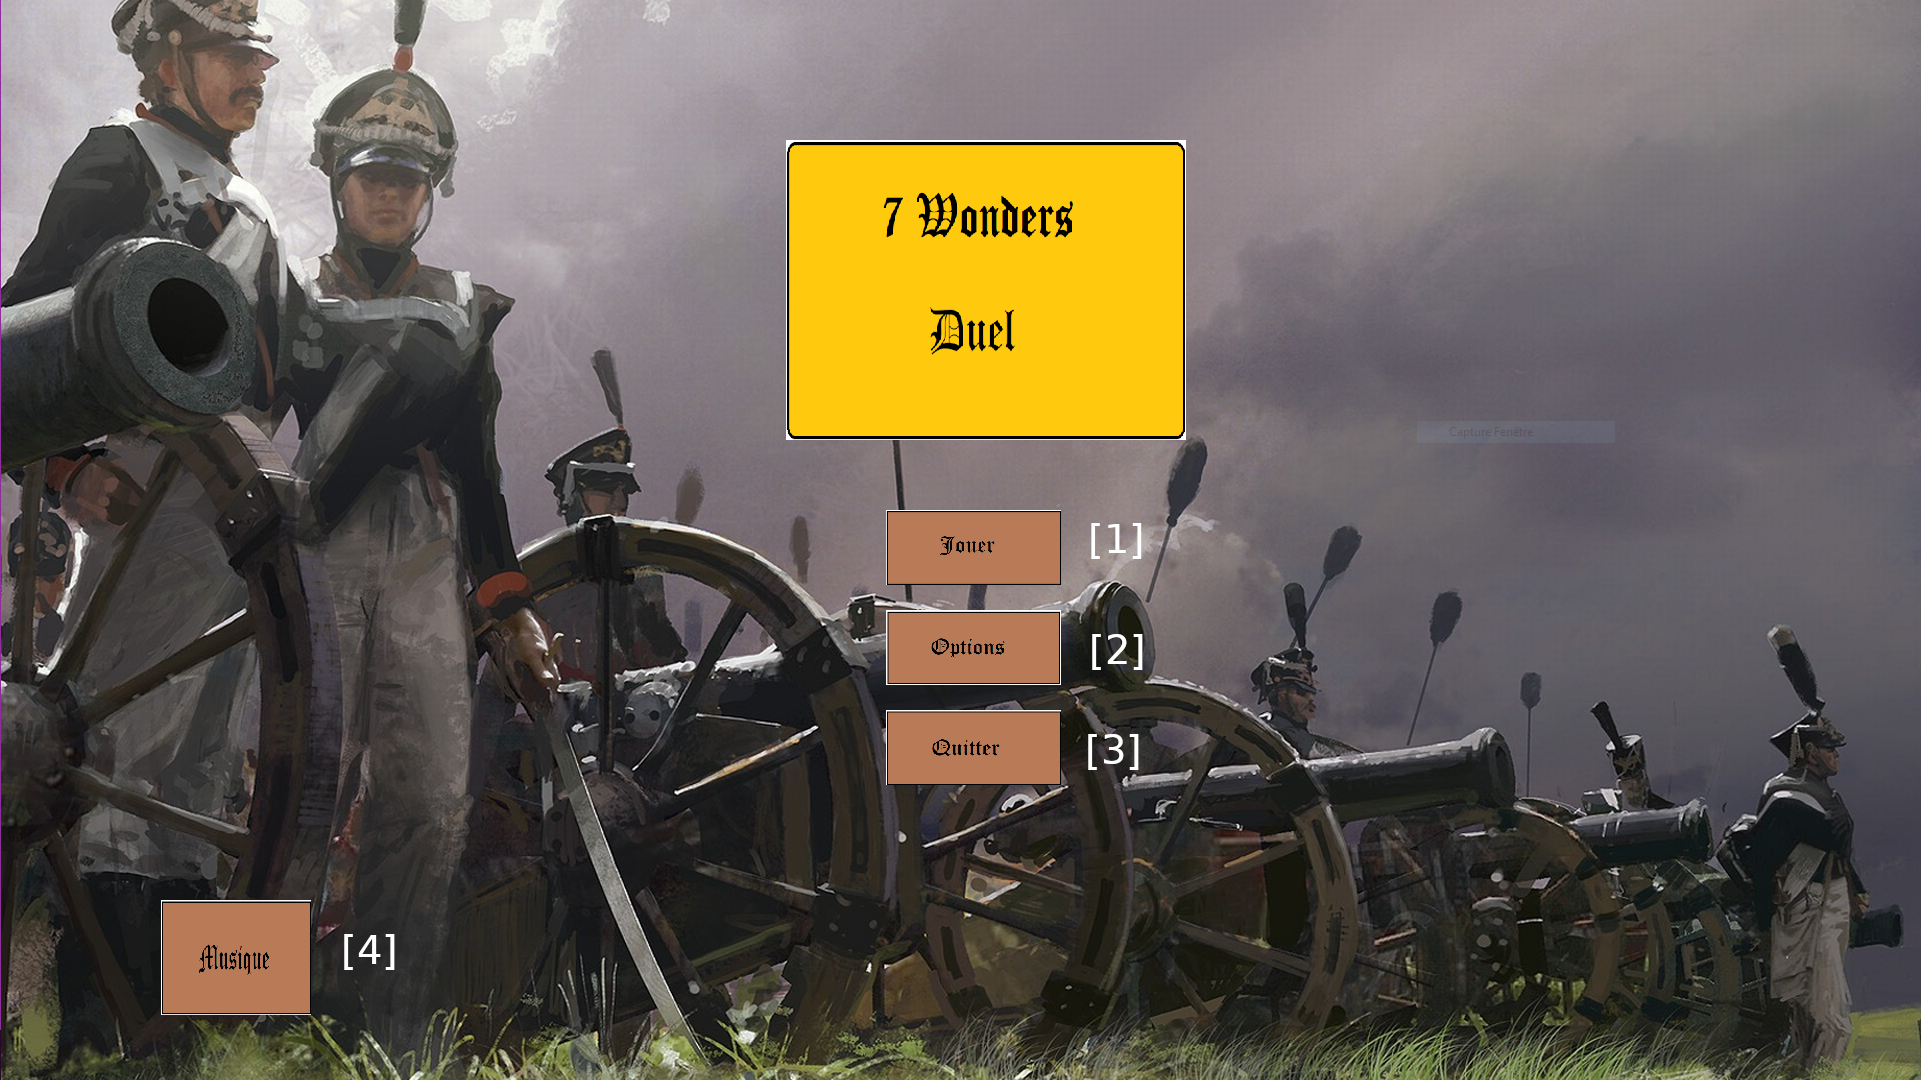
\includegraphics[width=.8\linewidth]{images/menu_principal.PNG}
            \caption{Menu principal}
        \end{figure}
        \newpage
	    Lorsque l'on clique sur le bouton pour jouer nous accèdons au deuxième menu. Celui ci contient le jeu (joueur contre ordi) [1], la selection de la difficultée [2] et un bouton pour revenir au menu principal [3]. 
	   % \begin{figure}[htbp]
    %         \centering
    %         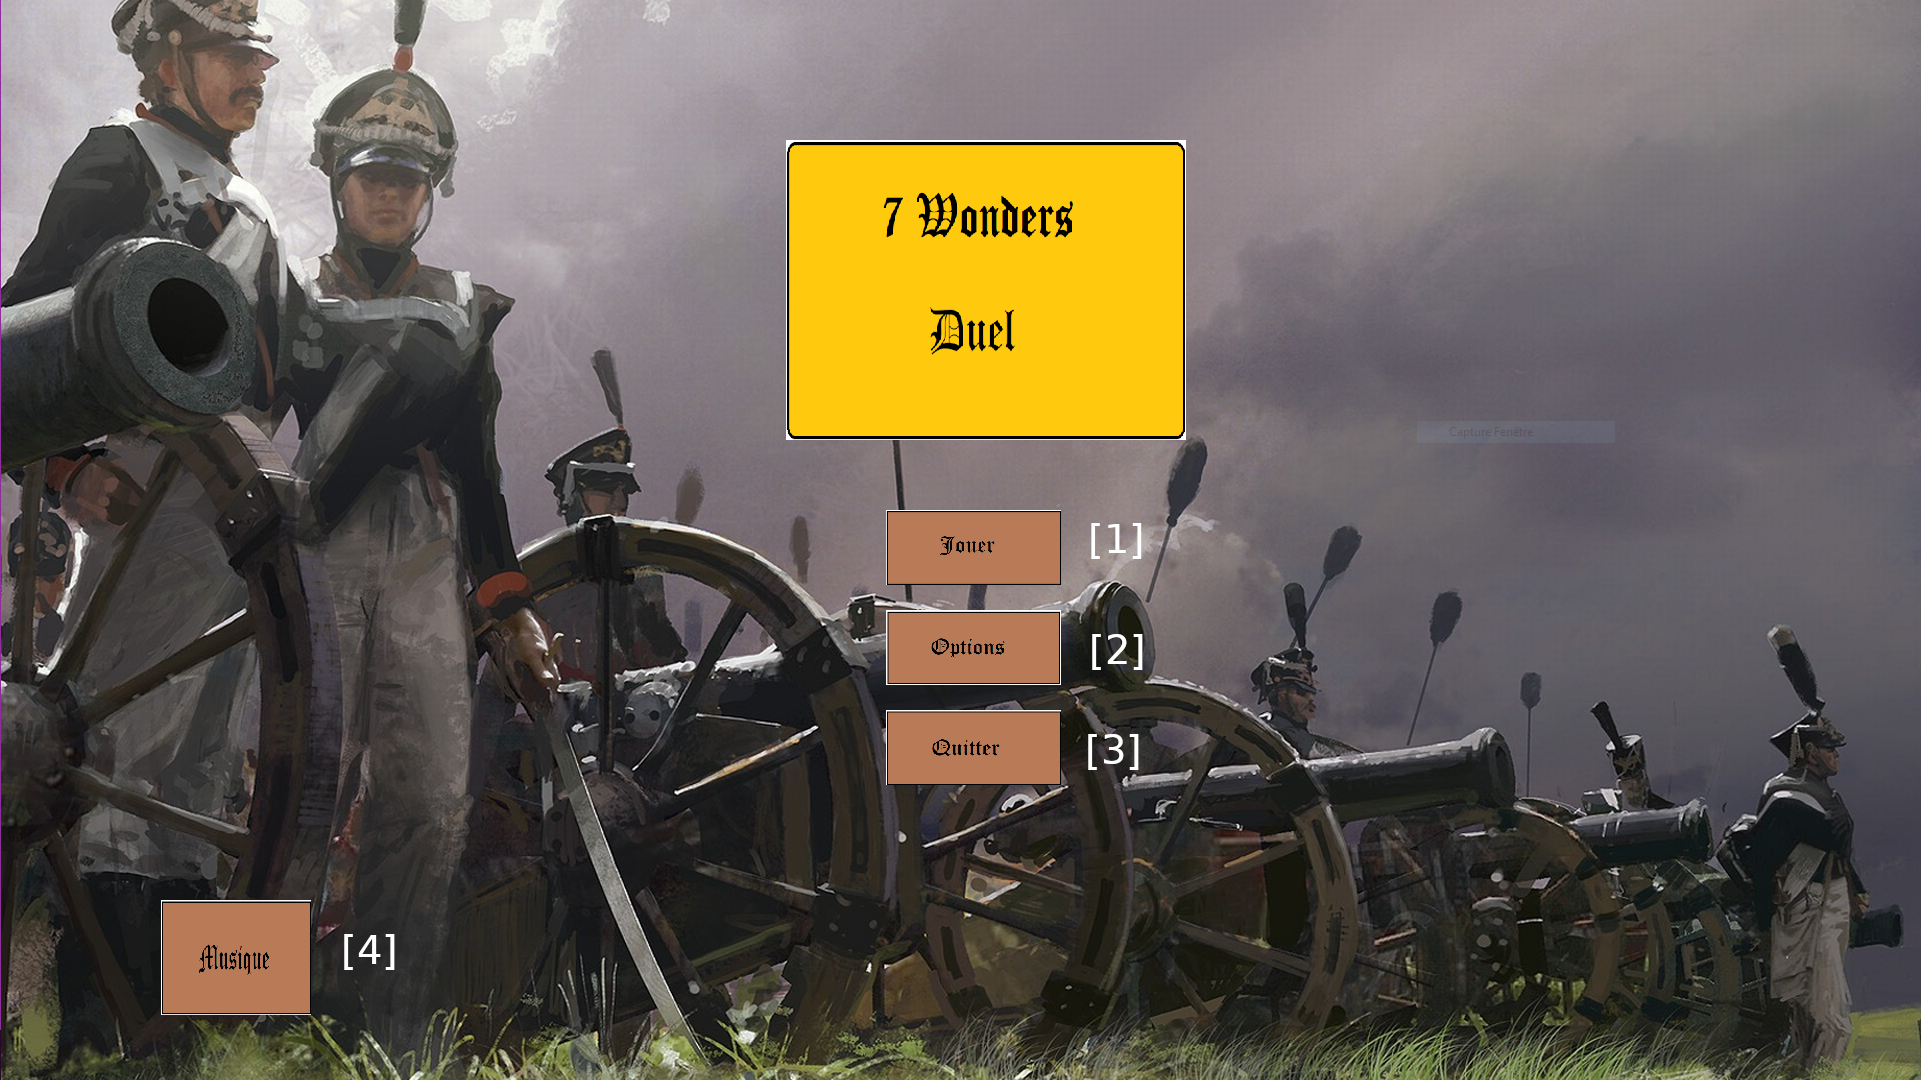
\includegraphics[width=.8\linewidth]{images/menu_principal.PNG}
    %         \caption{Menu principal}
    %     \end{figure}
	    Lorsque l'on clique sur le bouton pour le choix de la difficultée nous arrivons sur le menu pour selectionner la difficultée parmis facile, normal et difficile. 
	    \begin{figure}[htbp]
            \centering
            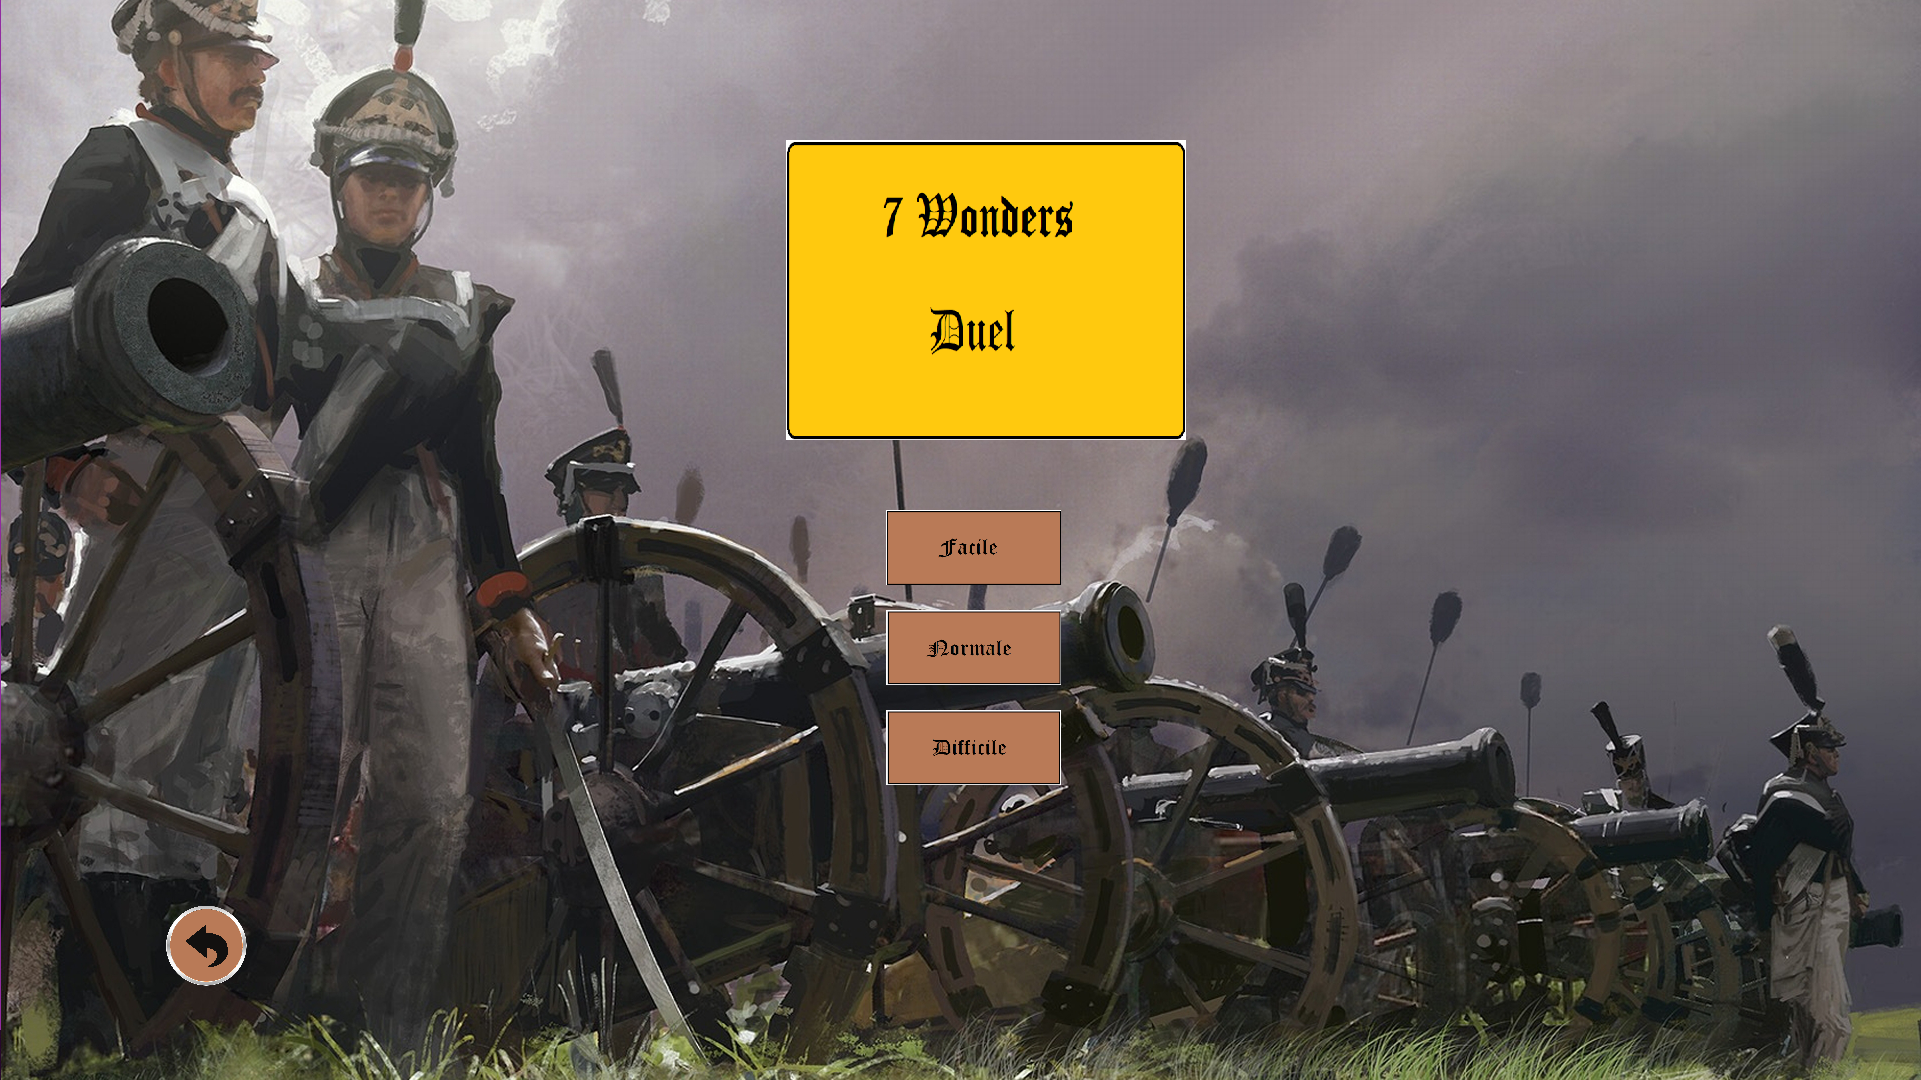
\includegraphics[width=.8\linewidth]{images/menu_difficultees.PNG}
            \caption{Menu des difficultées}
        \end{figure}
        \newpage
	    Enfin nous avons le jeu à proprement parlé.
	    \begin{figure}[htbp]
            \centering
            \begin{subfigure}{.55\textwidth}
                \includegraphics[width=\linewidth]{images/partie_age_I.PNG}
                \caption{Age I}
    	    \end{subfigure}
    	    \begin{subfigure}{.55\textwidth}
                \includegraphics[width=\linewidth]{images/partie_age_II.PNG}
                \caption{Age II}
    	    \end{subfigure}
    	    \begin{subfigure}{.55\textwidth}
                \includegraphics[width=\linewidth]{images/partie_age_III.PNG}
                \caption{Age III}
    	    \end{subfigure}
            \caption{Une partie de 7 Wonders-Duel}
        \end{figure}
	
% 	\subsection{Résultat obtenu}
    \newpage
	\section{Conclusion}
	    \subsection{Difficultée(s) rencontrée(s)}
    	Nous sommes rapidement tombés sur une première difficultée lorsque nous rédigions le schéma de classe du jeu. Par exemple, les cartes comportent beaucoup d'effets pouvant avoir un impact sur le joueur, comme un gain de ressource(s), mais aussi sur le jeu (gain d'agent auprès de la banque, le fait du pouvoir rejouer, ect). Cela implique que l'effet doit être appliqué par le jeu et non par le joueur, nous avons du changer nos schémas en conséquences.\\
    	Ensuite nous voulions créer des classes (plus précisément des interfaces) pour les effets (avec une interface "mère" pour que les cartes possèdent une liste d'objets de type "mère" spécialisé avec les différents effets) mais cela rendait compliqué la création d'effet puis la création de carte en leur associant les effets.\\
    	Comme nous avions choisit Python comme language nous avons décidé de faire au plus simple quitte à produire un code ne respectant pas les conventions de programmation et les patterns définis. Le code n'a pas pour but d'être mis à jour, le respect des patterns n'étaient pas une obligation. 
    	
    	La deuxième difficulté était lors de l'implémentation de la fonction d'évaluation, en particulier lors de l'implémentation. En effet le système de copie nous a donné beaucoup de fils a retordre. Cela fut aussi lonng à mettre en place car nous manipulons beaucoup d'objets (liste, dicionnaire, classes) imbriqués les uns dans les autres, il fallut être minucieux lors de l'implétation des constructeurs par copie. \\
    	Enfin les tests concernant nos notations de cartes furent compliqués à vérifier, même sur une petite profondeur (=3), à l'age I cela nous faisait quand même un grand nombre de calculs à faire à la main (6 cartes prenables, puis 5 cartes pour la réponse soit 30 calculs, parmis toutes les combinaisons de 17 cartes prisent aléatoirement).
	
	\subsection{Objectif(s) atteint/ non atteint}
	    Premièrement l'objectif concernant le jeu, nous avons réussi a implémentation la majeur partie des fonctionnalitées du jeu. Malheureusement par manque de temps, certains effets complexes ont été simplifié (le choix de l'utilisateur a été remplacé par un tirage aléatoire). Voici la liste complète des effets simplfiés : 
	    \begin{itemize}
	        \item ???
	    \end{itemize}
	    Concernant le rendu de l'application, nous avons réussi a reproduire le placement utilisé pour le jeu papier, cela donne un visuel très jolie. Cependant, l'affichage excessif d'élément sur le plateau cause des latences du à la bibliothèque graphique et le jeu comporte beaucoup d'élément ce qui donne un aspect "chargé" à l'application, nous avons fait notre possible pour répartir au mieux ces derniers.
	    % TODO : Deuxièmement l'objectif concernant le coeur du projet, la fonction d'évaluation.
	
	\subsection{Suggestion d'amélioration(s)}
	    Pour les améliorations, nous pouvons re-structuré le projet et les différents modules afin de respecter tous les patterns et les règles de programmation afin de rendre le code plus lisible et modifiable si l'on souhaite. Nous pouvons egalement trouver une autre bibliothèque graphique rendant le jeu plus rapide et moins consommateur de ressources. Nous devons finir les effets qui ont été simplifié pour respecter complètement les règles du jeu. 
	   % TODO : Nous pouvons également modifier la fonction d'évaluation pour rendre l'ordinateur plus "intelligent" dans ces coups.
	    
%     \newpage
% 	\section{Annexe}
% 	\subsection{Code}
        
    \newpage
	\printbibliography

\end{document} 